\documentclass[letterpaper]{report}

\usepackage[letterpaper,margin=0.75in,includefoot,footskip=30pt]{geometry}
\usepackage{layout}
\usepackage{multicol}
\usepackage[parfill]{parskip}
\usepackage{bibleref}
\usepackage[urlcolor=blue,colorlinks=true]{hyperref}
\usepackage{graphicx}
\graphicspath{ {IsraelWebImages/} }
\usepackage{float} % Allows the [H] to be used to avoid floating in multicol
\usepackage{caption}
\captionsetup[figure]{labelformat=empty} % Don't call figures "figures"

\title{Israel Pilgrimage}
\author{Jedidiah \& Tatiana Bartlett}
\date{}

%Use this command to add verse superscripts
\newcommand{\vs}[1]{\textsuperscript{#1}}

\begin{document}
\maketitle

%%%%%%%%%%%%%%%%%%%%%%%%%%%%%%%%%%%%%%%%%%%%%%%%%%%%%%%%%%%%%%%%%%%%%%%%%%%%%%%
%%%%%%%%%%%%%%%%%%%%%%%%%%%%%%%%%%%%%%%%%%%%%%%%%%%%%%%%%%%%%%%%%%%%%%%%%%%%%%%
\chapter{In Preparation}

\section{Preparation of This Document}
I wanted to do some deliberate preparation and pre-reading for the trip,
and typing it all out seemed like a good way to get that done.

\subsection{Fr. Gregory's Comments}
My Father-in-law was kind enough to send out some initial tips and thoughts
in several e-mails which  I consolidated here to form the framework of this 
document.

I left his notes intact here with only some grammatical enhancements and
embedding of the links to make it read a little nicer,
but otherwise it still reads as though he wrote it himself.

\subsection{Bible Verses}
The bible verses were copy-pasted from the website \url{https://www.biblegateway.com/}.

I selected the RSV translation since that seems to be the de-facto standard
for liturgical use, and I've had no major issues with the translation myself.

Using the website, it was really easy to just type in some verses and their
range, for example: \href{https://www.biblegateway.com/passage/?search=Matthew+2%3A13-23&version=RSV}{
Matthew 2:13-23}

\subsection{Additional Contemplation}
I also wanted to have a paragraph of historical context about what we would be
seeing on the trip,
so I included what seemed most relevant

\subsection{Journaling}
I left extra space for writing notes and thoughts for the day as they occurred 
to me,
as well as set the expectation that Tatiana and I would try to write down a
journal entry at the end of each day, so that we could re-read it at some 
point in the future and remember some forgotten detail or significant impact
that gets too easily forgotten in the waves of reality that will inevitably
ensue.

\section{The TODO list}
Before we left, Tatiana and I had a long checklist
of things that we needed to get done.

This included:
\begin{itemize}
    \item Getting our wills in order and ensuring our children and legacy would
    be cared for without causing undue burden on their guardians.
    \item Arranging for my mother to come and care for our children / animals / house while we are away.  This included:
    \begin{itemize}
        \item Buying a burner phone for my mom so she had emergency contact 
        capabilities (beyond using Google hangouts / skype for calling to
        Canada to keep in touch and for us to call back to her).
        \item Ensuring that she would be covered by our vehicle insurance
        \item Getting her on the phone list for school so she could know if 
        there was going to be cancellations
        (There's been at least 5 late-starts or total cancellations already 
        this year. Lots of snowfall in the 2016-2017 winter season)
        \item Having here come down early so that we can help show her our routine for the kids and where everything is.
        \item Providing her with emergency numbers for anything and everything.
    \end{itemize}
    \item Purchasing an international SIM card so that I can call/text while
    there for emergencies,
    as well as for uploading pictures and journaling
    directly to the cloud.
\end{itemize}

%%%%%%%%%%%%%%%%%%%%%%%%%%%%%%%%%%%%%%%%%%%%%%%%%%%%%%%%%%%%%%%%%%%%%%%%%%%%%%%
%%%%%%%%%%%%%%%%%%%%%%%%%%%%%%%%%%%%%%%%%%%%%%%%%%%%%%%%%%%%%%%%%%%%%%%%%%%%%%%
\chapter{The Journey}
%%%%%%%%%%%%%%%%%%%%%%%%%%%%%%%%%%%%%%%%%%%%%%%%%%%%%%%%%%%%%%%%%%%%%%%%%%%%%%%
\section{Jan 24 - Tuesday - Arrival Day}
Arrive in Tel Aviv and travel to and Check-in at Bethlehem

\subsection{Notes from Fr. Gregory}
We will arrive in the late afternoon at Ben Gurion Airport in Tel Aviv.
By the time we clear customs, we will be quite tired and ready to transfer by bus 
to our hotel in Bethlehem.
(Originally this was the Grand Park Hotel, but I can't recall if our tour 
director told me that this had to be changed.
I am forwarding this to him as well for final clarification).


We will have dinner and rest at the hotel in Bethlehem in preparation for our
big first day.

\subsection{Daily Notes}

\subsection{Journal Entry}

%%%%%%%%%%%%%%%%%%%%%%%%%%%%%%%%%%%%%%%%%%%%%%%%%%%%%%%%%%%%%%%%%%%%%%%%%%%%%%%
\clearpage
\section{Jan 25 - Wednesday - Day 1}
Feast of St. Gregory the Theologian

\subsection{Notes from Fr. Gregory}
We may be able to celebrate Liturgy this day. We shall see if this is possible. Either way, we will visit: the Church of the Nativity with Grotto beneath (spot where Christ was born); Grotto of the Holy Innocents; Shepherds' Fields (Ancient Byzantine Church remnant)...the Gospel passages for these sites are: 
Matthew 1:18-25; Matthew 2:1-12; Matthew 2:13-23; Luke 2:1-20

You may also study a bit more about the Holy Innocents on the
\href{https://oca.org/saints/lives/2007/12/29/103682-14000-infants-the-holy-innocents-slain-by-herod-at-bethlehem}{
    OCA website - Holy Innocents Slain By Herod at Bethlehem}. 

After lunch (remember, you have paid for three meals each day),
we will take taxis to St. Sabbas Monastery in the desert.
While women are not permitted in the monastery,
special provisions are made for them to be able to see down into the courtyard 
and (the last time I was here),
to venerate the Holy Relics. You can learn more about the monastery at
\href{http://stsabbas.org/jerusalem.html}{stsabbas.org}\footnote{If you poke 
    around on this site,
    you will find some important visitor etiquette that will 
    be beneficial for all of the Orthodox monasteries}
or at the \href{https://en.wikipedia.org/wiki/Mar_Saba}{
    Wikipedia page for Mar Saba}.

Read more about the 
\href{https://oca.org/saints/lives/2008/12/05/103477-venerable-sava-the-sanctified}{The Life of St. Sabbas} before we arrive.

We will then return to the hotel in Bethlehem for dinner and rest...

\subsection{Church of the Nativity}
\begin{multicols}{2}

\subsubsection{\href{https://en.wikipedia.org/wiki/Church_of_the_Nativity}{
Church of the Nativity - Wikipedia}}

The Church of the Nativity is a basilica located in Bethlehem, West Bank.

The church was originally commissioned in 327 by Constantine the Great and his 
mother Helena over the site that was traditionally considered to be located 
over the cave that marks the birthplace of Jesus.
The Church of the Nativity site's original basilica was completed in 339 and 
destroyed by fire during the Samaritan Revolts in the 6\textsuperscript{th} century.
A new basilica was built 565 by Justinian, the Byzantine Emperor,
restoring the architectural tone of the original.
The site of the Church of the Nativity has had numerous additions since this 
second construction, including its prominent bell towers.
Due to its cultural and geographical history,
the site holds a prominent religious significance to those of the Christian faith.

The site of the Church of the Nativity is a World Heritage Site,
and was the first to be listed under Palestine by the United Nations Educational,
Scientific and Cultural Organization (UNESCO). The site is also on UNESCO's List of World Heritage in Danger.

\begin{figure}[H]
\centering
\label{fig:GrottoOfTheNativity}
\caption{Grotto Of The Nativity}
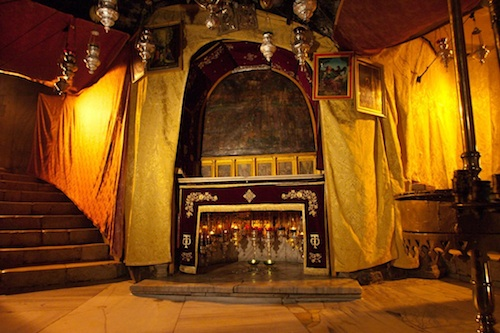
\includegraphics[width=\columnwidth]{GrottoOfTheNativity}
\end{figure}

\subsubsection{\href{http://www.bethlehem.custodia.org/default.asp?id=469}{
Church of the Nativity - bethlehem.custodia.org}}

The entrance today is placed sideways with respect to the location where Jesus was born, but it is thought that in the fourth century the entrance was located behind the presbytery. The small façades of the two side entrances date back to the times of the Crusaders.
The Grotto is entered by descending the stairs to the right of the iconostasis. Here the space is very narrow and restricted and the walls, which were originally irregular, form an almost-rectangular perimeter. The natural walls of the cave, decorated in the Constantine period, were covered with marble during the Byzantine period.
The Altar of the Nativity only began to be venerated in the Byzantine period when this space was created to commemorate the precise place in which Jesus had been born.
The current structure has been totally modified from that which was described by the pilgrim John Phocas and Abbot Daniel in the 12th century. Two red stone columns, and the inscription “Gloria in excelsis Deo et in terra pax hominibus”, overlook the altar, above which are representations of the Virgin and the Child in swaddling clothes, the scene of the washing, and that of the coming of the shepherds.
Beneath the altar is a star with the inscription “Hic de Virgine Maria Iesus Christus natus est” in memory of the precise spot of the Nativity. To the right of the altar is the place where Mary laid Jesus in the manger, also known as the Crib. At this point in the Grotto the floor is lower and the space is made up of columns similar to the Byzantine ones in the nave of the church, and by the remains of two Crusader columns.
In front of the Crib is a small altar dedicated to the Magi, where the Latins celebrate Holy Mass. The structure of the Crib is not the original one but is the result of alterations necessitated by the continuous wear and tear of time and the passage of pilgrims.
Following the fire of 1869 the walls of the Grotto were covered with asbestos to prevent further fires, a donation from the President of the French Republic Marshal Mac-Mahon in 1874. Below this covering the original Crusader marble is still visible, while above it can be seen wood panel paintings of limited artistic value.

\end{multicols}

\subsection{Scripture}

{\centering
\emph{\bibleverse{Matthew}(1:18-25) The Birth of Jesus the Messiah}\\
}
\begin{multicols}{2}
\vs{18}Now the birth of Jesus Christ took place in this way.
When his mother Mary had been betrothed to Joseph,
before they came together she was found to be with child of the Holy Spirit;
\vs{19}and her husband Joseph,
being a just man and unwilling to put her to shame,
resolved to divorce her quietly.
\vs{20}But as he considered this,
behold, an angel of the Lord appeared to him in a dream, saying,
``Joseph, son of David, do not fear to take Mary your wife,
for that which is conceived in her is of the Holy Spirit;
\vs{21}she will bear a son, and you shall call his name Jesus,
for he will save his people from their sins.''

\vs{22}All this took place to fulfill what the Lord had spoken by the prophet:

\begin{verse}
\vs{23}``Behold, a virgin shall conceive\\
and bear a son,\\
and his name shall be called Emman′u-el''\\
(which means, God with us).\\
\end{verse}

\vs{24}When Joseph woke from sleep,
he did as the angel of the Lord commanded him;
he took his wife,
\vs{25}but knew her not until she had borne a son;
and he called his name Jesus.
\end{multicols}

{\centering
\emph{\bibleverse{Matthew}(2:1-12) The Visit of the Wise Men}\\
}
\begin{multicols}{2}
\vs{1}Now when Jesus was born in Bethlehem of Judea in the days of Herod the king,
behold, wise men from the East came to Jerusalem, saying,
\vs{2}``Where is he who has been born king of the Jews?
For we have seen his star in the East, and have come to worship him.''
\vs{3}When Herod the king heard this, he was troubled, and all Jerusalem with him;
\vs{4}and assembling all the chief priests and scribes of the people,
he inquired of them where the Christ was to be born. \vs{5}They told him, ``In Bethlehem of Judea; for so it is written by the prophet:

\begin{verse}
\vs{6}`And you, O Bethlehem,\\
in the land of Judah,\\
are by no means least among the rulers of Judah;\\
for from you shall come a ruler\\
who will govern my people Israel.' ''\\ 
\end{verse}

\vs{7}Then Herod summoned the wise men secretly and ascertained from them what
time the star appeared;
\vs{8}and he sent them to Bethlehem, saying,
``Go and search diligently for the child,
and when you have found him bring me word,
that I too may come and worship him.''
\vs{9}When they had heard the king they went their way;
and lo, the star which they had seen in the East went before them,
till it came to rest over the place where the child was.
\vs{10}When they saw the star, they rejoiced exceedingly with great joy;
\vs{11} and going into the house they saw the child with Mary his mother,
and they fell down and worshiped him.
Then, opening their treasures, they offered him gifts,
gold and frankincense and myrrh.
\vs{12}And being warned in a dream not to return to Herod,
they departed to their own country by another way.
\end{multicols}

\subsection{Grotto of the Holy Innocents}
\begin{multicols}{2}

\subsubsection{\href{http://www.bethlehem.custodia.org/default.asp?id=473}{
Holy Innocents - bethlehem.custodia.org}}

With our back to the Altar of St. Joseph,
to our right is the Grotto of the Innocents in which one can see three 
arcosolium (or “bench”) type tombs,
each containing from two to five sepulchers.

Here the Massacre of the Innocents ordered by Herod the Great shortly after 
Jesus’ birth is commemorated.
In the first centuries, the memory of the Innocents was commemorated in an
adjoining cave,
which one can assume was a common grave in which numerous bones of corpses had 
been found.

\begin{figure}[H]
\centering
\label{fig:GrottoOfTheInnocents}
\caption{Grotto Of The Holy Innocents}
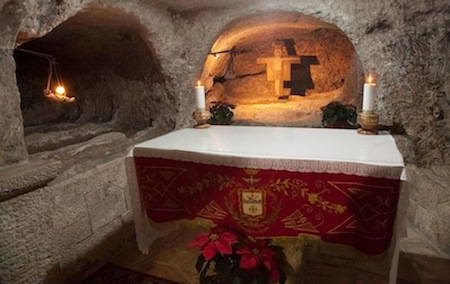
\includegraphics[width=\columnwidth]{GrottoOfTheInnocents}
\end{figure}

\end{multicols}

\subsubsection{Scripture}
{\centering
\emph{\bibleverse{Matthew}(2:13-23) The Escape to Egypt,
The Massacre of the Infants,
The Return from Egypt}\\
}
\begin{multicols}{2}
\vs{13}Now when they had departed, behold,
an angel of the Lord appeared to Joseph in a dream and said, ``Rise,
take the child and his mother, and flee to Egypt,
and remain there till I tell you; for Herod is about to search for the child,
to destroy him''
\vs{14}And he rose and took the child and his mother by night,
and departed to Egypt,
\vs{15}and remained there until the death of Herod.
This was to fulfill what the Lord had spoken by the prophet,
``Out of Egypt have I called my son.''

\vs{16}Then Herod, when he saw that he had been tricked by the wise men,
was in a furious rage,
and he sent and killed all the male children in Bethlehem and in all that 
region who were two years old or under,
according to the time which he had ascertained from the wise men.
\vs{17}Then was fulfilled what was spoken by the prophet Jeremiah:

\begin{verse}
\vs{18}``A voice was heard in Ramah,\\
wailing and loud lamentation,\\
Rachel weeping for her children;\\
she refused to be consoled,\\
because they were no more''\\
\end{verse}

\vs{19}But when Herod died, behold,
an angel of the Lord appeared in a dream to Joseph in Egypt, saying,
\vs{20}``Rise, take the child and his mother, and go to the land of Israel,
for those who sought the child’s life are dead.''
\vs{21}And he rose and took the child and his mother,
and went to the land of Israel.
\vs{22}But when he heard that Archela′us reigned over Judea in place of his 
father Herod, he was afraid to go there,
and being warned in a dream he withdrew to the district of Galilee.
\vs{23}And he went and dwelt in a city called Nazareth,
that what was spoken by the prophets might be fulfilled,
``He shall be called a Nazarene.''
\end{multicols}

\clearpage
\subsection{Shepherds' Fields}
\begin{multicols}{2}

\subsubsection{\href{http://www.custodia.org/default.asp?id=1888}{
Shepherds' Fields - Background}}

Some shepherds, amongst the most despised of the Jewish people,
went to adore Jesus. Dazzled by a great light,
an angel brought them the tidings of joy that the long-awaited Saviour had
been born.
And they heard a host of angels praising God who,
by sending the Messiah to the earth,
had shown His greatness to the celestial court and given salvation to men.

The Sanctuary, designed by Barluzzi, stands on a rock overlooking the ruins.
It has a dodecagonal shape with five apses having an inclined plane,
recalling the structure of a field tent like the one used by the shepherds at 
that time.
The light that penetrates the concrete and glass dome,
illuminating the interior calls to mind the divine light that appeared to the 
shepherds.

\begin{figure}[H]
\centering
\label{fig:ChurchOfTheAngelsAtShepherdsFields}
\caption{The Church of the Angels at Shepherd's Fields}
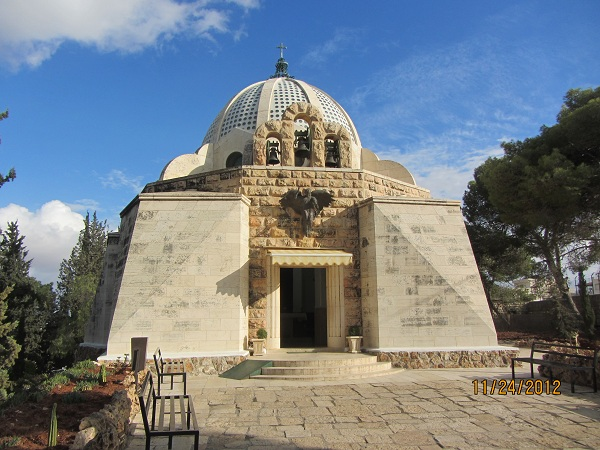
\includegraphics[width=\columnwidth]{ChurchOfTheAngelsAtShepherdsFields}
\end{figure}

\end{multicols}

\subsubsection{Scripture}
{\centering
\emph{\bibleverse{Luke}(2:1-20) The birth of Jesus, The Shepherds and the Angels}\\
}
\begin{multicols}{2}
\vs{1}In those days a decree went out from Caesar Augustus that all the world
should be enrolled.
\vs{2}This was the first enrollment, when Quirin′i-us was governor of Syria.
\vs{3}And all went to be enrolled, each to his own city.
\vs{4}And Joseph also went up from Galilee, from the city of Nazareth,
to Judea, to the city of David, which is called Bethlehem,
because he was of the house and lineage of David,
\vs{5}to be enrolled with Mary, his betrothed, who was with child.
\vs{6}And while they were there, the time came for her to be delivered.
\vs{7}And she gave birth to her first-born son and wrapped him in swaddling
cloths, and laid him in a manger,
because there was no place for them in the inn.

\vs{8} And in that region there were shepherds out in the field,
keeping watch over their flock by night.
\vs{9}And an angel of the Lord appeared to them,
and the glory of the Lord shone around them,
and they were filled with fear.
\vs{10}And the angel said to them, ``Be not afraid; for behold,
I bring you good news of a great joy which will come to all the people;
\vs{11}for to you is born this day in the city of David a Savior,
who is Christ the Lord.
\vs{12}And this will be a sign for you:
you will find a babe wrapped in swaddling cloths and lying in a manger.''
\vs{13}And suddenly there was with the angel a multitude of the heavenly host 
praising God and saying,

\begin{verse}
\vs{14}``Glory to God in the highest,\\
and on earth peace among men with whom he is pleased!''\\
\end{verse}

\vs{15}When the angels went away from them into heaven,
the shepherds said to one another,
``Let us go over to Bethlehem and see this thing that has happened,
which the Lord has made known to us.''
\vs{16}And they went with haste, and found Mary and Joseph,
and the babe lying in a manger.
\vs{17}And when they saw it they made known the saying which had been told
them concerning this child;
\vs{18}and all who heard it wondered at what the shepherds told them.
\vs{19}But Mary kept all these things, pondering them in her heart.
\vs{20}And the shepherds returned,
glorifying and praising God for all they had heard and seen,
as it had been told them.
\end{multicols}

\clearpage
\subsection{Daily Notes}

\clearpage
\subsection{Journal Entry}

%%%%%%%%%%%%%%%%%%%%%%%%%%%%%%%%%%%%%%%%%%%%%%%%%%%%%%%%%%%%%%%%%%%%%%%%%%%%%%%
\clearpage
\section{Jan 26 - Thursday - Day 2}

\subsection{Notes from Fr. Gregory}
We will have breakfast at the hotel and then take all of our luggage with us as we check out of the first hotel. Today we drive to Jerusalem, which is not that far away from Bethlehem. This morning we will be in the area of the Mount of Olives and the Garden of Gethsemane. Our sites will include several Russian Orthodox monasteries...one on the Mount of Olives and one at Gethsemane, the Tomb of the Holy Mother of God, and perhaps the Chapel of the Ascension. All of the sites on this day are outside of the walls of the Old City and we will have beautiful views of Jerusalem from these heights.

For the Mount of Olives, the Epistle and Gospel passages to be read are from the Ascension (Acts of the Apostles 1:1-12 and Luke 24:36-53). Here is a good site for the Chapel of the Ascension

\url{http://www.sacred-destinations.com/israel/jerusalem-chapel-of-ascension}

St. Pelagia the Penitent's Tomb is also here...we will need to ask the guard at the Chapel of the Ascension if we wish to see and venerate it...

Her life is here

\url{http://www.antiochian.org/node/16762}

Here is a very interesting site highlighting the history of the Mount of Olives, including the present day Russian Mission located there. This includes the Chapel of St. John the Baptist, built over the site where his honorable head was discovered.

\url{http://www.pravoslavie.ru/english/46854.htm}

And here is a history of the Russian Convent on the Mount of Olives

\url{http://jerusalem-mission.org/convent_ascension.html}

In this area are also the Dominus Flevit (The Lord Wept) Chapel, Church of the Pater Noster (Our Father) and the Church of All Nations. You may look those up as well and we will try to visit them if we have the time.

In general, the scriptures concerning Christ's Agony in the Garden of Gethsemane are Matthew 26:36-56; Mark 14:32-50; Luke 22:40-53; John 18:1-12.

We will also visit the Russian Orthodox Convent of St. Mary Magdalene in Gethsemane. The relics of Grand Duchess Elizabeth and the Nun Barbara are housed here. To read about this site, go here:

\url{http://www.pravoslavie.ru/english/63239.htm}

Hopefully, the sisters can tell us a little about the traditional location of Christ's Weeping in the Garden and why the monastery was built here.

Finally, we cannot forget the Tomb of the Holy Mother of God...it is also here, right next to the Church of All Nations. Here is a site highlighting that Holy Place:

\url{https://orthodoxword.wordpress.com/2010/08/15/the-tomb-of-the-most-holy-virgin-jerusalem/}

I also wish to make it a point to visit the relatively new Greek Orthodox Church of the Protomartyr Stephen, built near the site of his traditional martyrdom by stoning...the account of his martyrdom can be found in Acts of the Apostles 6:8-7:5, 46-60.

After Lunch, we will visit the Greek Orthodox Monastery of the Holy Cross which you can visit here

\url{http://www.biblewalks.com/Sites/CrossMonastery.html}

We are also scheduled to visit the Village of Ein Karem (Gornya) on this day...specifically, the Greek Orthodox Church of St. John the Baptist...read about this village here

\url{https://www.holyland-pilgrimage.org/ein-karem-home-of-john-the-baptist-and-place-of-the-visitation}

One other thought for this day...what a blessing to visit Katamon (The Monastery of St. Simeon the God-Receiver)...we shall try to do our best to see these Holy Places given our time restraints. Read the story of St. Simeon the God-Receiver in the Holy Scriptures at Luke 2:25-38. Here is a short description of the site...

\url{http://www.goisrael.com/Tourism_Eng/Tourist%20Information/Christian%20Themes/Details/Pages/St.%20Simeon%E2%80%99s%20Monastery%20chr.aspx}

I believe that we will stay at the Golden Walls Hotel in Jerusalem on this night...so we will check in and have dinner there...rest up because we have only toured for two days (and just describing these two days has already made me tired)!!!

\subsection{Daily Notes}

\clearpage
\subsection{Journal Entry}

%%%%%%%%%%%%%%%%%%%%%%%%%%%%%%%%%%%%%%%%%%%%%%%%%%%%%%%%%%%%%%%%%%%%%%%%%%%%%%%
\clearpage
\section{Jan 27 - Friday - Day 3}

\subsection{Notes from Fr. Gregory}
On Day 3 we will enter the old city of Jerusalem through the Dung Gate. We will go to the Temple Mount and see the Western Wall (last remaining piece of the Old Temple)...as well as the Dome of the Rock. It may be possible, while at the Temple Mount (Sion), to visit the Upper Room and even King David's Tomb...we will check on these sites when we get on the ground over there. Holy Scripture: Mark 14:12-26; Matthew 26:17-30; John 13:1-17 and (Pentecost) Acts 2:1-21.

Next we will be on the Via Dolorosa (Way of the Cross)...this is the traditional path taken by Christ as He carried the Holy Cross to Golgotha...it includes the Lithostrotos (Flagellation Chapel) and a good explanation is here

\url{http://www.mikemasonbooks.com/the-lithostrotos-chapter-57-of-jesus-his-story-in-stone/}

In this vicinity is the Sheep's Pool (Bethesda)...read the Gospel of John 5:1-15 and, while I am thinking of pools, just outside of the Old City is Siloam...read John 9:1-38. We shall try to get there as well. Before getting to the Holy Sepulchre, there remains the Church of St. Anne and the Monastery of Sts. Joachim and Anna...you can look here

\url{http://www.seetheholyland.net/church-of-st-anne/}

and here, respectively, for some background  (the following is a video, with Greek chanting)

\url{http://www.johnsanidopoulos.com/2011/09/video-home-of-sts-joachim-and-anna-in.html}

After lunch, we are scheduled to Greek Orthodox Patriarchate of Jerusalem and, if the Lord blesses it, to receive the Blessing of the Patriarch of Jerusalem. Following this, we will visit the holiest site in all of Christendom...the Church of the Holy Sepulchre. There is too much here to describe. Here are SOME (not all) of the relevant Gospel passages covered beneath the roof of this incredible Holy Place: Mark 15:43-47 (The Anointing Stone inside the entrance); Matthew 27:27-56 (Golgotha...each evangelist has a passage announcing this); and the Life-Giving Tomb of Christ...Mark 15:42-16:8 (each evangelist also joyously announces this reality as well). Here is link that should give us a pretty good start:
\url{https://orthodoxwiki.org/Church_of_the_Holy_Sepulchre_(Jerusalem)}

We then return for dinner and overnight to our hotel in Jerusalem.


\subsection{Daily Notes}

\clearpage
\subsection{Journal Entry}

%%%%%%%%%%%%%%%%%%%%%%%%%%%%%%%%%%%%%%%%%%%%%%%%%%%%%%%%%%%%%%%%%%%%%%%%%%%%%%%
\clearpage
\section{Jan 28 - Saturday - Day 4}

\subsection{Notes from Fr. Gregory}
After breakfast, we depart for the Monastery of St. Gerasimos...here is a nice little feature to give everyone some background about this saint and this site:

\url{http://www.biblewalks.com/Sites/StGerassimos.html}

or

\url{http://www.seetheholyland.net/monastery-of-st-gerasimus/}

(This monastery is built over the site believed to house a cave where the Holy Family stayed as they fled to Egypt and is also famous for being the monastery of St. Zosimas, who traveled into the desert and met St. Mary of Egypt).

We then travel to Qasr el-Yahud where we will visit the Jordan River and celebrate the Outdoor Blessing of Water...some people enjoy actually entering the river completely and being blessed with these holy waters. (Matthew 3:13-17; Mark 1:9-11; Luke 3:21-23.

Anyone who might wish to experience "swimming" in the Dead Sea (more like floating) should be prepared to do it on this day...in other words, swim atire would be good today.

After lunch in Jericho, we will visit the Tree of Zacchaeus and Monastery of the Prophet Elijah, Luke 19:1-10; Monastery of the Mount of Temptation (Luke 4:1-14) and Monastery of St. George in Wadi Qelt (Elijah's Cave) (we will walk down if time permits)...

\url{https://en.wikipedia.org/wiki/St._George's_Monastery,_Wadi_Qelt}

We return to the hotel for dinner and a little rest before departing for Liturgy at the Holy Sepulchre (optional) to be there by 11pm for the Liturgy at Midnight...time may vary.

\subsection{Daily Notes}

\clearpage
\subsection{Journal Entry}

%%%%%%%%%%%%%%%%%%%%%%%%%%%%%%%%%%%%%%%%%%%%%%%%%%%%%%%%%%%%%%%%%%%%%%%%%%%%%%%
\clearpage
\section{Jan 29 - Sunday - Day 5}

\subsection{Notes from Fr. Gregory}
We check out of the hotel in Jerusalem and head for Bethany to visit the Church and Tomb of Lazarus and the Monastery of Martha and Mary. John 11:1-45

After Lunch in Samaria, we visit Sebastia (Nablus)...Jacob's Well and Prison of St John the Baptist (John 4:5-42 and Mark 6:14-29. Go to

\url{https://en.wikipedia.org/wiki/Jacob's_Well}

We will then continue to the city of Tiberias on the Sea of Galilee for dinner and overnight at the Ron Beach Hotel.


\subsection{Daily Notes}

\subsection{Journal Entry}

%%%%%%%%%%%%%%%%%%%%%%%%%%%%%%%%%%%%%%%%%%%%%%%%%%%%%%%%%%%%%%%%%%%%%%%%%%%%%%%
\clearpage
\section{Jan 30 - Monday - Day 6}

\subsection{Notes from Fr. Gregory}
After breakfast, we will visit the Greek Orthodox Churches of Sts. Peter and Paul in Tiberias and the Church of the Apostles in Capernaum (site of the healing of the paralytic). Read Mark 2:1. -12. We may also visit other sites in Capernaum (Mark 1:21-31). After lunch, we will visit Tabgha and the Church of the Loaves and Fishes (Matthew 14:14-21 or John 6:5-14). We also visit the Mount of the Beatitudes (Matthew 5:1-12). We finish the day with a boat ride across the Sea of Galilee back to our hotel in Tiberias.


\subsection{Daily Notes}

\clearpage
\subsection{Journal Entry}

%%%%%%%%%%%%%%%%%%%%%%%%%%%%%%%%%%%%%%%%%%%%%%%%%%%%%%%%%%%%%%%%%%%%%%%%%%%%%%%
\clearpage
\section{Jan 31 - Monday - Day 7}
This is our final full day in the Holy Land...see how fast the time has gone?

\subsection{Notes from Fr. Gregory}
After breakfast, we drive to Nazareth. On the way, we will stop at Cana, the site of Christ's first miracle (John 2:1-12). In Nazareth, (Luke 1:24-38), we will visit the site of the Annunciation, where Christ, our God, became a man.  After lunch, we will ascend Mount Tabor where Christ was transfigured before His Holy Apostles...Luke 9:28-36; Matthew 17:1-9. The us will take us to the bottom of the Mountain and taxis will take us up to the top. Finally, we go back to the hotel in Tiberias for dinner and overnight in preparation for our early departure the next morning! Glory be to God!

\subsection{Daily Notes}

\clearpage
\subsection{Journal Entry}

%%%%%%%%%%%%%%%%%%%%%%%%%%%%%%%%%%%%%%%%%%%%%%%%%%%%%%%%%%%%%%%%%%%%%%%%%%%%%%%
%%%%%%%%%%%%%%%%%%%%%%%%%%%%%%%%%%%%%%%%%%%%%%%%%%%%%%%%%%%%%%%%%%%%%%%%%%%%%%%
\chapter{Reflections}
%%%%%%%%%%%%%%%%%%%%%%%%%%%%%%%%%%%%%%%%%%%%%%%%%%%%%%%%%%%%%%%%%%%%%%%%%%%%%%%
\section{Feb 1}


\end{document}
